\setcounter{equation}{0}
Функция $\frac{1}{R} = \frac{1}{\sqrt{(x - \xi)^2 + (y - \eta)^2 + (z - \zeta)^2}}$, представляющая потенциал поля единичной массы (заряда), помещённой в точке $M_0(\xi, \eta, \zeta)$ является решением уравнения Лапласа, зависящим от параметров $\xi$, $\eta$, $\zeta$. Интегралы от этой функции по параметрам называются \textit{потенциалами} и имеют существенное значение с точки зрения непосредственных приложений в физике, а так же и с точки зрения развития методов решения краевых задач.\\

\begin{wrapfigure}{l}{0.3\textwidth}
	\centering
	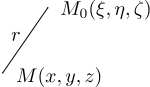
\includegraphics{figPotentialTheo1.pdf}
\end{wrapfigure}
Пусть в некоторой точке $M_0(\xi, \eta, \zeta)$ помещена масса $M$. По закону всемирного тяготения на массу $m$, помещённую в точке $M(x, y, z)$, действует сила притяжения
\[
	F = - \gamma \frac{mM}{R^2} r
\]
где $r = \frac{1}{R}$ --- единичный вектор в направлении $\overrightarrow{M_0M}$, а $\gamma$ --- гравитационная постоянная. 
Сила называется потенциальной, если существует функция, через которую она выражается как градиент некоторой потенциальной фукнции:
\[
	F = \mathrm{grad} \Pi
\]
Покажем, что при $\gamma M = 1$ сила выражается так
\[
	F = \mathrm{grad} \left(\frac{m}{r} \right)
\]
Силовое поле описывается потенциалом $\frac{m}{r}$. Если будет $n$ точек, то $\sum\limits_{i=1}^n \frac{M_i}{r_i}$. \\
Если масса распределена непрерывно, то 
\[
	\iiint\limits_{\omega} \frac{\rho (\xi, \eta, \zeta)}{\sqrt{(x - \xi)^2 + (y - \eta)^2 + (z - \zeta)^2}}\, d\omega
\]

В дальнейшем $\rho$ мы будем называть плотностью потенциала. Плотность может распределяться не только по объёму, но и по поверхности. Помимо объёмного потенциала будем рассматривать поверхностный потенциал:
\[
	\iint\limits_S \frac{\nu(\xi, \eta, \zeta)}{r}\, dS;
\]
\[
	\iint\limits_S \mu (\xi, \eta, \zeta) \derp{}{\vec n}{} \frac{1}{R}\, dS.
\]
где $\nu, \mu$ --- плотности.
Особая точка $(\xi, \eta, \zeta)$. Тогда $\Omega = \omega_1 + \omega_2$.\\
\[
	V_1 = \iiint\limits_{\omega_1} \quad V_2 = \iiint\limits_{\omega_2}
\]
Рассмотрим объём $V_2$:
\begin{multline*}
	\derp{V_2}{x}{2} + \derp{V_2}{y}{2} + \derp{V_2}{z}{2} = \iiint\limits_{\omega_2} \rho(\xi, \eta, \zeta) \left(\derp{}{x}{2} \left(\frac{1}{r} \right)  \right)  + \derp{}{y}{2} \left(\derp{}{x}{2} \left(\frac{1}{r} \right) \right)  +  \derp{}{z}{2} \left(\derp{}{x}{2} \left(\frac{1}{r} \right) \right) d\omega_2 = 0
\end{multline*}
Теперь рассмотрим $V_1$:
\[
	\derp{V}{x}{} = \iiint\limits_{\omega_1} \rho_0 (\xi, \eta, \zeta) \derp{}{x}{} \left(\frac{1}{r} \right)\, d \omega_1
\]
Аналогично по $y$ и по $z$:
\[
	\derp{}{x}{} \left(\frac{1}{r} \right) = - \frac{1}{r^2} \derp{r}{x}{} = - \frac{1}{r^3} (x \xi) = - \derp{}{\xi}{} \left(\frac{1}{r} \right)
\]
Функция $\rho$ --- непрерывная по $\Omega$.
\begin{multline*}
	 \derp{V}{x}{} = - \iiint\limits_{\omega_1} \rho (\xi, \eta, \zeta) \derp{}{\xi}{} \left(\frac{1}{r} \right)\, d\omega_1 = - \iiint\limits_{\omega_1} \left[\derp{}{\xi}{} \left(\rho \frac{1}{r} \right) - \frac{1}{r} \derp{\rho}{\xi}{}\right]\, d\omega_1 = \\
	 - \iiint\limits_{\omega_1} \derp{}{\xi}{} \left(\frac{\rho}{r} \right)\, d\omega_1 + \derp{\rho_{\text{сред}}}{\xi}{}  \int\limits_0^{2\pi} d \varphi \int\limits_0^{ \pi} d\theta \frac{1}{\varepsilon} \varepsilon^2 \sin \theta =
\end{multline*}

\begin{wrapfigure}{l}{0.2\textwidth}
	\centering
	\includegraphics{figPotentialTheo2.pdf}
\end{wrapfigure}
$\varepsilon$ --- радиус малой сферы $\omega_1 \to 0$. Применим теорему Остроградского--Гаусса и перейдём к интегралу по поверхности:
\[
	 = - \iint\limits_{s_1} \frac{\rho}{r} \cos d S_1
\]
$\alpha$ --- угол между $n$ и $x$.


\begin{align*}
	&\derp{V}{x}{2} = - \iint\limits_{s_1} \rho(\xi, \eta, \zeta) \cos \alpha \derp{}{x}{} \left(\frac{1}{r} \right) dS_1 = \iint\limits_{S_1} \frac{\rho(\xi, \eta, \zeta) \cos \alpha}{r^2} \cos \theta dS_1 = - \iint\limits_{S_1} \frac{\rho(\xi, \eta, \zeta) \cos^2 \alpha}{r^2}\, dS_1\\
	&\derp{V}{y}{2} = - \iint\limits_{S_1} \frac{\rho(\xi, \eta, \zeta) \cos^2 \beta}{r^2}\, dS_1\\
	&\derp{V}{z}{2} = - \iint\limits_{S_1} \frac{\rho(\xi, \eta, \zeta) \cos^2 \gamma}{r^2}\, dS_1
\end{align*}



\[
	\delta V = \derp{V}{x}{2} + \derp{V}{y}{2} + \derp{V}{z}{2} = - \iint\limits_{S_1} \frac{\rho(\xi, \eta, \zeta)}{r^2} (\cos^2 \alpha + \cos^2 \beta + \cos^2 \gamma) dS_1 =  - \iint\limits_{S_1} \frac{\rho(\xi, \eta, \zeta)}{r^2}\, dS_1 
\]
Воспользуемся теоремой о среднем:
\[
	 - \iint\limits_{S_1} \frac{\rho(\xi, \eta, \zeta)}{r^2} dS_1 = - \rho_{\text{ср}}(\xi, \eta, \zeta) \int\limits_0^{2 \pi} \int\limits_0^{\pi} \frac{1}{\varepsilon^2} \sin \theta \varepsilon^2\, d \theta = - 4 \pi \rho(\xi, \eta, \zeta)
\]
Обозначим $\rho = \frac{f}{4 \pi}$ и поулчим:
\[
	\Delta V = \Delta V_2 + \Delta V_2 = - f
\]
Объёмный потенциал является решением неоднородного уравнения Лапласа.
\[
	V= \frac{1}{4 \pi} \iiint\limits_{\omega} \frac{f(\xi, \eta, \zeta)}{r} d\Omega
\]
Теперь рассмотрим поверхностный интеграл.\\
Потенциал простого слоя:
\[
	\iint\limits_S \mu(\xi, \eta) \frac{1}{r}\, dS
\]
Потенциал двойного слоя:
\[
	\iint\limits_S \nu (\xi, \nu) \derp{}{n}{} \left(\frac{1}{r} \right)\, dS
\]\\


Вспомним формулу Грина:
\[
	\iint\limits_S \left(u\derp{G}{n}{} - G \derp{u}{n}{}  \right) d S - \iiint\limits_\omega (u \Delta G - G \Delta u) d\Omega = \begin{cases}
		4 \pi u &\mbox{внутри}\\
		2 \pi u &\mbox{на границе}\\
		0 &\mbox{снаружи}
	\end{cases}.
\]
Пусть $G = \frac{1}{r}$ в качестве возьмём $u = \nu_0$
\[
	\Delta \nu_0 = 0 \qquad \derp{\nu_0}{n}{} = 0
\]
\[
	\nu_0 = - \frac{1}{4 \pi} \iint\limits_{\nu_0} \derp{}{n}{} \left(\frac{1}{r} \right)\, dS
\]
\[
	\iint\limits_S \left(\nu_0 \derp{}{n}{} \left(\frac{1}{r} \right) \right)\, dS = \begin{cases}
		4 \pi \nu_0 \\
		2 \pi \nu_0 \\
		0 
	\end{cases}
\]
\[
	W_{\text{в}}^0 = - \frac{1}{4 \pi} \iint\limits_S \nu_0 \derp{}{n}{} \left( \frac{}{n} \right)\, dS
\]
\[
	W_{\text{ср}}^0 = - \frac{1}{2 \pi} \iint\limits_S \nu_0 \left(\frac{1}{r} \right)\, dS
\]
\[
	W_{\text{н}}^0 = 0
\]\\

\[
	W_{\text{в}}^0 = W_0 + 2 \pi \nu_0
\]
\[
	W_{\text{н}}^0 = W_0 - 2 \pi \nu_0
\]
При переходе через границу потенциал двойного слоя терпит разрыв
\[
	I = \iint\limits_S (\nu - \nu_0) \derp{}{n}{} \left(\frac{1}{r} \right) dS = \iint\limits_{S_1} (\nu - \nu_0) \derp{}{n}{} \left(\frac{1}{r} \right) dS + \iint\limits_{S-S_1} (\nu - \nu_0) \derp{}{n}{} \left(\frac{1}{r} \right) dS
\]
\[
	 \iint\limits_S (\nu - \nu_0) \derp{}{n}{} \left(\frac{1}{r} \right) dS \leqslant \varepsilon \iint\limits_{S_1} \derp{}{n}{} \left(\frac{1}{r} \right)\, dS 
\]
\[
	\varepsilon \iint\limits_{S_1} \derp{}{n}{} \left(\frac{1}{r} \right)\, dS = - \varepsilon \iint\limits_{S_1} \frac{\cos \alpha}{r^2}\, dS = - \varepsilon \int\limits_0^{2 \pi} d\varphi \int\limits_0^\pi \sin \theta\, d\theta
\]
\begin{multline*}
	W_{\text{в}} = \iint\limits_S \left[\nu \derp{}{n}{} \frac{1}{r} - \nu_0 \derp{}{n}{} \frac{1}{r} + \nu_0 \derp{}{n}{} \frac{1}{r} \right] dS =
\iint\limits_S \nu_0 \derp{}{n}{} \frac{1}{r} dS = I + W_{\text{в}}^0 = \underbrace{I + W_0(\nu_0)}_{W_0(\nu)} - 2 \pi \nu_0
\end{multline*}

\[
	W_{\text{в}} = W_0(\nu) - 2 \pi \nu
\]
\[
	W_{\text{н}} = W_0(\nu) + 2 \pi \nu
\]
\[
	W_{\text{в}}(M)  = \iint\limits_S \nu \derp{}{n}{} \frac{1}{r} - 2 \pi \nu \big|_S
\]
\[
	\Delta W = 0 \quad W = - \iint\limits_S \nu(\xi, \eta) \derp{}{n}{} \frac{1}{r} dS
\]
на границе  $W|_S = f$\\
\[
	W_{\text{в}} = \iint\limits_S \nu \derp{}{n}{} \frac{1}{r} - 2 \pi \nu = f
\]

\begin{equation}
	\nu(P_0) - \frac{1}{2 \pi} \iint\limits_S \nu(P) \derp{}{n}{} \frac{1}{r} dS = - \frac{1}{2 \pi} f (P_0)
	\label{equ:equUnique1}
\end{equation}
Уравнение \eqref{equ:equUnique1} является уравнением Фредгольма 2-го рода.

Из него можем определить плотности поверхностного потенциала $\nu$
\[
	W_{\text{в}} = \oint \nu \derp{}{n}{} \left(\ln \frac{1}{r} \right) dl
\]
\[
	\nu(P_0) - \frac{1}{\pi} \oint \nu (P) \derp{}{n}{} \left(\ln \frac{1}{r} \right) dl = - \frac{1}{\pi} f (P_0)
\]
\[
	W_{\text{в}} - \oint \nu \derp{}{n}{} \left(\ln \frac{1}{r} \right)
\]
На границе должно выполняться:
\[
	\nu (p_0) - \frac{1}{\pi} \oint \nu(p) \derp{}{n}{} \left(\ln \frac{1}{r} \right)\, dl = - \frac{1}{\pi} f(p_0)
\]
